\section{Аль-Хорезми}
\subsection{Биография}
Начнем с обсуждения аль-Хорезми, отца алгебры. Абу Абдулла Мухаммад ибн Муса Аль-Хорезми жил около 800-847 н.э., но эти даты неточны. Эпитет «аль-Хорезми» относится к его месту происхождения, Хорезму или Хорезму, который расположен к югу от дельты реки Аму-Дарья и Аральского моря в Центральной Азии. Однако историк аль-Табари добавляет эпитет «аль-Кутруббулли», указывая, что аль-Хорезми в действительности прибыл из Кутрубулла, недалеко от Багдада между реками Тигр и Евфрат. Другие источники утверждают, что, возможно, предки аль-Хорезми, а не он сам, происходят из Хорезма. Еще одним интересным эпитетом, добавленным аль-Табари, является «аль-Маюси», что означало бы, что аль-Хорезми был приверженцем Зороастрийская религия. Однако предисловие аль-Хорезми к его трактату о альберте не вызывает сомнений, что он был набожным мусульманином; возможно, некоторые из его предков или даже аль-Хорезми в юности были зороастрийцами.

Аль-Хорезми вырос под Багдадом под властью Калифа аль-Мамуна (царствование 813-833 гг. Н.э.), который был великим пропагандистом науки. Аль-Хорезми была предложена должность в Байт-аль-Хикме (Дом Мудрости) в Багдаде; большинство его трактатов посвящено халифу аль-Мамуну.

\subsection{Математический вклад Аль-Хорезми}
\subsubsection{Астрономия}
Большинство трактатов аль-Хорезми относятся к области астрономии. Он был одним из разработчиков астролябии, а также составил примерно сотню астрономических таблиц. Одна из этих таблиц, Зидж Аль-Синдхинд (перевод индийской работы, Зидж — общее название для астрономических таблиц в странах ислама.), является первой арабской астрономической работой из всех которые сохранились. 

\subsubsection{География}
Он также написал текст географии, Китаб сурат аль-ард, в котором перечислены долготы и широты городов и населенных пунктов. Это было основано на карте мира аль-Мамуна, на которой работал аль-Хорезми, которая, в свою очередь, была основана на географии Птолемея. Однако карта мира аль-Мамуна была гораздо более точной, чем Птолемея, особенно в отношении исламского мира.

\subsubsection{Календарь}
Еще одна сохранившаяся работа аль-Хорезми - это его работа над еврейским календарем, в котором точно описывается 19-летний цикл, семь месяцев и правила определения, в какой день недели начинается месяц Тишри. Он также подсчитывает интервал между еврейской эрой или созданием Адама и эры Селуддида, которая началась 1 октября 312 года до нашей эры. Также, аль-Хорезми включает метод определения средней долготы Солнца и Луны.


\subsubsection{Арифметика}
В дополнение к его работам по алгебре, трактаты аль-Хорезми, которые обеспечили его прочную славу, - его работы по арифметике. Его арифметический трактат, возможно, озаглавлен «Китаб аль-иам ва'л-тафрик би-абаб аль-Хинд», или «Книга добавления и вычитания» по методу расчета индусов. Однако оригинальная арабская рукопись теперь потеряна, и его текст сохранился только в ее латинском переводе, который, возможно, сделал Аделард из Бата в 12 веке. Впервые он был опубликован в 1857 году в журнале «Algoritmi de numero indorum» Б. Бонкомпаньи, а затем опубликован в 1963 году как «Алгоритм Мохаммеда ибн Муса Альхваризми» Курта Фогеля. Это первый известный учебник о десятичной системе, и это первый трактат который систематически излагает использование арабских (или иногда индусско-арабских) цифр 1-9, 0 и позиционной системы счисления.\cite{mohamed} Ввод в использование числа 0 было самым важным; «маленький круг на самом деле является одной из величайших математических инноваций в мире».\cite{mohamed} Символ 0 использовался около 250 лет в исламском мире после его введения аль-Хорезм прежде чем западный мир когда-либо узнал об этом.

Современная цифровая нотация, безусловно, имеет свои корни в аль-Хорезми и других арабских математиках; хотя под влиянием индуистских цифр аль-Хорезми и его арабские преемники ввели полную концепцию десяти чисел и метод десятичных обозначений\cite{mohamed}. Аль-Хорезми представил ноль, и его способ счисления индийских цифр был настолько точными, что он, вероятно, был ответственен за распространенное мнение о том, что наша система счисления - арабская. Хотя аль-Хорезми никогда не претендовал на оригинальность в отношении своей системы чисел, латинские переводы его произведений были широко распространены в Европе, а неосторожные читатели приписывали автора и нумерацию автору\cite{boyer}. Именно эта связь с числами привело к искажению имени аль-Хорезми к алгоризму, что, в свою очередь, привело к современному слову алгоритм.

\subsection{Алгебра Аль-Хорезми}
\subsubsection{Аль-джабр и Аль-мукабала}
В интересах этой статьи наиболее важной темой будет трактат аль-Хорезмита \textit{Китаб аль-джабр ва'л-мукабала}, или \textit{Книга восстановления и балансировки} \cite{boyer}. Значения слов \textit{аль-джабр} и \textit{аль-мукабалах} обсуждаются. Аль-джабр, которое пришло к нам в форме «алгебры», вероятно, имелось в виду нечто вроде «восстановления» или «завершения», ссылающееся на перенос членов на другую сторону уравнения с отрицательным знаком или добавление одинаковых членов к обоим сторонам уравнения чтобы устранить отрицательные члены \cite{boyer}. Аль-мукабала, вероятно, означает нечто вроде «восстановления» или «балансировки», ссылаясь на вычеркивание подобных членов с противоположных сторон уравнения или уменьшение положительных членов на вычитание равных значений из обеих сторон уравнения\cite{boyer}, 257. Вместе два слова аль-джабр и аль-мукабала могут означать науку об алгебре. В трактате Аль-Хорезми была первая книга, в которой этот титул обозначался как отдельная дисциплина.

Может быть полезно увидеть примеры того, как аль-Хорезми использовали эти термины. Он сначала ставит проблему:

\begin{displayquote}
Я разделил десять на две части. Я умножил одну из двух частей на другую. После этого я умножил одну из частей саму на себя. Результат умножения само на себя в четыре раза больше, чем произведение одной из частей на другую.\cite{vanderwaer}
\end{displayquote}

Аль-Хорезми называет одну из частей «вещь», а другую «десять минус вещь. Он умножает на два, получает «десять вещей минус квадрат», а затем получает (в современных обозначениях):

$$x^2 = 40x - 4x^2$$

Он использует \textit{аль-джабр} для добавления $4x^2$ к обеим сторонам, что дает:

$$5x^2 = 40x$$

Аль-Хорезми затем получает

$$x^2 = 8x$$

из которого он получает

$$x = 8$$

(Для современного читателя очевидно, что аль-Хорезми не допускает $x$
равным $0$)

На другой странице у аль-Хорезми есть уравнение:

$$50 + x^2 = 29 + 10x$$

Он использует \textit{аль-мукабалах}, чтобы вычесть из обоих сторон $29$, чтобы получить:

$$21 + x^2 = 10x$$

\subsubsection{Происхождение алгебры}
Важно отметить, что \textit{Происхождение алгебры} уходит корнями к древним египтянам и вавилонянам, у которых были тексты, посвященные проблемам арифметики, алгебры и геометрии еще в 2000 году до нашей эры. В «Арифметике» Диофанта уже появилось несколько уравнений. Однако эти уравнения были решены как часть решений других проблем и не подвергались систематической обработке. Аль-Хорезми был первым, кто систематически изучал алгебру. Хотя существовали уравнения Диофанта, аль-Хорезми, вероятно, не знал о них в то время, когда писал свой трактат; аль-Хорезми не знал греческого языка, и в то время не было арабского перевода Арифметики. На Аль-Хорезми, вероятно, больше влияли индуистские или местные сирийско-персидско-еврейские источники. Однако ни один из этих источников не перешел к аль-Хорезми; несколько текстов, которые, по-видимому, были написаны после Китаб аль-Джабра ва'л-мукабала. Некоторые западные исследователи утверждают, что Аль-Хорезми не является «настоящим математиком», поскольку «в его работе мало того, чего нельзя найти в более ранних индийских источниках».

\subsubsection{Алгебраические уравнения}
\textit{Китаб аль-джаб ва'л-мукабала} состоит из трех секций, первая из которых утверждает, что все линейные и квадратичные уравнения могут быть сведены к одному из шести типов:

$$ax^2 = bx$$
$$ax^2 = b$$
$$ax = b$$
$$ax^2 + bx = c$$
$$ax^2 + c = bx$$
$$ax^2 = bx + c$$

Он представляет общие решения для всех этих типов. Рассматривая эти шесть уравнений, очевидно, что аль-Хорезми не принимал отрицательные или нулевые коэффициенты.

Трактаты Аль-Хорезми о смешанных квадратичных уравнениях («корни и числа, равны квадратам», «квадраты и числа, равны корням») лучше всего рассматривать на примере первого типа смешанных квадратичных уравнений. В словах аль-Хорезми:


\begin{displayquote}
\textit{Корни и квадраты, равны числам}
Например: один квадрат и десять корней одного и того же значения равны тридцати девяти дирхемов; то есть, какова должна быть площадь, которая, если ее увеличить на десять собственных корней, составляет тридцать девять?

Решение: вы сокращаете вдвое количество корней, которые в данном примере дают пять. Это вы умножаете само на себя; произведение составляет двадцать пять. Добавьте это к тридцати девяти; сумма составит шестьдесят четыре. Теперь возьмите корень этого, который равен восьми, и вычтите из него половину числа корней, что равно четырем. Отстаток три. Это корень площади, о которой вы думали; сам квадрат равен девяти.
\end{displayquote}

В современных обозначениях уравнение имеет вид:

$$x^2 + 10x = 39$$

и решение Аль-Хорезми это:

$$(x + 5)^2 = 39 + 25 = 64$$
$$x + 5 = \sqrt{64} = 8$$
$$x = 8 -5 = 3$$
$$x^2 = 9$$

Ал-Хорезми демонстрирует это решение с помощью квадрата $AB$, стороной которого является искомый корень x. На каждой из четырех сторон он строит прямоугольники, каждый из которых имеет ширину 2.5. Итак, квадрат вместе с четырьмя прямоугольниками равен 39. Чтобы заполнить квадрат $EH$, аль-Хорезми добавляет четыре раза квадрат 2.5 или 25. Таким образом, площадь большого квадрата $EH$ равна 64, а его сторона равна 8 Таким образом, сторона x исходного квадрата $AB$ равна $8 - 5 = 3$ (см. рисунок ниже).

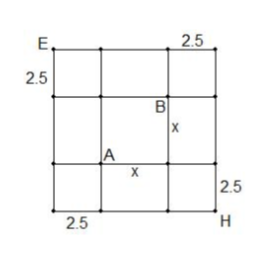
\includegraphics[scale=0.5, center]{1}

Аль-Хорезми также представляет более простой похожий метод, который строит прямоугольники ширины 5 с двух сторон квадрата $AB$. Тогда общая площадь квадрата $EH$ равна $x^2 + 10x + 25 = 39 + 25 = 64$, что дает тот же результат $x = 3$ или $x^2 = 9$ (см. рисунок ниже).

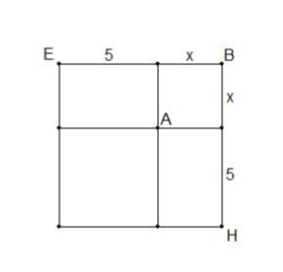
\includegraphics[scale=0.5, center]{2}

Аль-Хорезми также обсуждает методы извлечения квадратного корня; этот метод, возможно, был адаптирован из индуистских источников. Этоn метод проще всего объяснить на примере. Чтобы найти квадратный корень из 107584, «вертикальные линии нарисованы и цифры разбиты на периоды по две цифры». Ближайший корень из 10 равен 3, и поэтому его квадрат равный 9 вычитается из 10. 3 написанно ниже всего, как часть окончательного квадратного корня. 3 удваивается, чтобы сделать 6, что содержится дважды в 17; $6 \times 2 = 12$, поэтому 12 вычитается из 17 что оставляет 5. Таким образом, 2 записывается внизу как следующая часть окончательного квадратного корня. Затем квадрат 2 (который равен 4) вычитается из 55, что дает в остатке 51. Таким образом, 518 затем делится на двойное 32 (что равно 64), оставляя 8. Таким образом, $8 \times 64 = 512$ вычитается из 518 оставляя 6. Последняя цифра тогда равна 64, что составляет 8 в квадрате, поэтому последняя цифра конечного квадратного корня равна 8. Следовательно, квадратный корень из 107584 равен 328. (рисунок ниже).

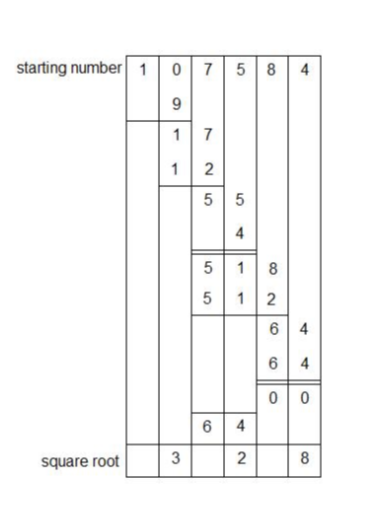
\includegraphics[scale=0.5, center]{3}

\subsubsection{Мероопределение}
Вторая глава \textit{Алгебры} Аль-Хорезми относится к вопросу о мерах. В нем изложены правила для вычисления площадей и объемов. Площадь круга можно найти, умножив половину диаметра на половину окружности. Чтобы найти окружность, аль-Хорезми предоставляет три правила.

С диаметром $d$ и окружностью $p$ и приблизительным значением $\pi = p / d$:

$$p = 3\frac{1}{7}d\textrm{, или } \pi \approx 3.1439$$
$$p = \sqrt{10d^2}d\textrm{, или } \pi \approx 3.1639$$
$$p = \frac{62832}{20000}d\textrm{, или } \pi \approx 3.1416$$

Первое правило было сформулировано Архимедом и также было дано в \textit{Метрике} Герона Александрийского и в еврейском трактате \textit{Мишнат ха-Миддот}. Второе приведенное правило можно найти в \textit{Брахмашфутасиддханте} Брахмагупты. Третий (эквивалентный точной оценке $\pi \approx 3.1416$) приписывается «Астрономам» Аль-Хорезми, который может относиться к индусскому астроному Ариабхате; то же правило можно найти в его «Арябхатии».

Аль-Хорезми также утверждает, что для прямоугольного треугольника со сторонами $a$, $b$ $c$, с «короткими» сторонами $a$ и $b$:

$$a^2 + b^2 = c^2$$

Он дает доказательство в тексте; однако его доказательство справедливо только для равностороннего треугольника, когда $a = b$. Из этого видно, что основной источник Аль-Хорезми не может быть классическим греческим трактатом, таким как \textit{Начала} Евклида. Еврейский трактат \textit{Мишнат ха-Миддот} тесно связан с главой Аль-Хорезми о измерениях, которая показывает какую-то прямую зависимость или общий источник обоих. Если Соломон Гандс прав, автор еврейского трактата был раввином Неемии, который жил около 150 г. н.э., Аль-Хорезми, возможно, полагался на трактат или на перевод или текст перевода в Перине или Сирии. Однако другие авторы быстро указывают на то, что вывод Соломона Гандса не подтвержден, что оставляет дату появления Мишнат ха-Миддо открытым даже до того периода, когда аль-Хорезми опубликовал свою Алгебру. Гад Сарфатти утверждает, что Мишнат ха-Миддот был написан не позднее позднего исламского периода и может быть адаптацией работы Аль-Хорезми.

\subsubsection{Наследия}
Последняя глава Алгебры является самой большой. Она целиком состоит из задач и решений, включающих простые арифметические и линейные уравнения. Эти проблемы не будут обсуждаться здесь, поскольку они используют ту же самую алгебру, которая уже обсуждалась.

\subsubsection{Влияние}
Алгебра Аль-Хорезми стала известна, как только она была опубликована, и мусульманские математики прокомментировали ее во время жизни Аль-Хорезми. Алгебра впервые стала известной на Западе, когда европейские ученые, такие как Аделард Бат (1120 г.) и Роберт Честер (1140 г.), начали переводить арабские произведения на латынь. Леонардо Пизанский, также известный как Фибоначчи, включает в себя многие задачи, связанные с Аль-Хорезми. Однако они, скорее всего, взяты из текстов Абу Камиля, в которых используются многие проблемы и решения Аль-Хорезми. Уильям Луна, еще один итальянский математик, перевел Алгебру Аль-Хорезми на итальянский язык в начале 13 века; на этот перевод ссылались несколько ученых в 16 веке. Влияние трактата Аль-Хорезми достигло работ Иоганнеса де Муриса в 14-м веке, Regiomontanus в 15 веке, а Адам Ризе, Перес де Мойя , Кардана и Адриан Ромена в 16 веке. Даже сегодня некоторые учителя элементарной алгебры используют предложения, уравнения и геометрические представления Аль-Хорезми, даже не зная их источника. Мохини Мохамед очень хорошо подытоживает прочное влияние аль-Хорезми, и поэтому я оставляю ее заключение:

\begin{displayquote}
Во момент его смерти наследие, которое Аль-Хорезми оставил в исламском сообществе, включало способ представления чисел, который привел к удобному методу вычисления, даже с дробями; наука об алгебре; и карту мира, которая является более точной, чем когда-либо прежде.

В западном мире математическая наука была более подвержена влиянию аль-Хорезми, чем любой другой средневековый писатель. Именно благодаря Аль-Хорезми мы можем широко использовать арабские цифры. Позиционная система счисления по основанию 10, свободное использование иррациональных чисел и его введение алгебры в современном смысле сделали его главной фигурой в истории мусульманской математики. Его введение арабских цифр изменило содержание и характер математики и произвело революцию в обычной практике расчета в Средневековой Европе. С интеграцией греческой, индуистской и, возможно, вавилонской математики в его алгебре этот текст является одним из лучших представлений международного символа исламской средневековой цивилизации. Среди прочего, слова алгебра, алгоритм, шифр и корень выжили в качестве свидетелей роли Аль-Хорезми в создании и распространении науки вычислений.
\end{displayquote}




